\documentclass[conference]{IEEEtran}
% The preceding line is only needed to identify funding in the first footnote. If that is unneeded, please comment it out.
\usepackage{cite}
\usepackage{amsmath,amssymb,amsfonts}
\usepackage{algorithmic}
\usepackage{graphicx}
\usepackage{textcomp}
\usepackage{xcolor}
\def\BibTeX{{\rm B\kern-.05em{\sc i\kern-.025em b}\kern-.08em
    T\kern-.1667em\lower.7ex\hbox{E}\kern-.125emX}}
\begin{document}

\title{Summary of “An Investigation into Android In-App Ad Practice: Implications for App Developers”  \\
}

\author{\IEEEauthorblockN{Stephane Meunier}
\IEEEauthorblockA{\textit{Department of Mathematics and Computer Science} \\
\textit{Clark University}\\
Worcester, Massachusetts \\
smeunier@clarku.edu}
\and
\IEEEauthorblockN{Catalin Veghes}
\IEEEauthorblockA{\textit{Department of Mathematics and Computer Science} \\
\textit{Clark University}\\
Worcester, Massachusetts \\
cveghes@clarku.edu}
}

\maketitle

\begin{abstract}
The purpose of this paper is to summarize the work\cite{ReferencePaper} conducted by Boyuan He, Haitao Xu, Ling Jin, Guanyu Guo, Yan Chen, and Guangyao Weng during their research which was published in IEEE INFOCOM 2018 Conference.

In-app advertising represents the major source of income for millions of developers and application owners. To monetize their mobile apps, these people commonly utilize various ad networks and ad types to generate revenues in order to sustain their products. Even though it is a widespread habit, especially among free applications which do not charge users for downloading the software, there are neither formal studies nor recommendations about this segment’s best practices. The conference paper under discussion strives to reveal suitable implementations for advertisements and provide stakeholders guidelines on ad network selection and ad placement to maximize income without affecting the overall user experience. While working on this paper, the authors investigated 277,616 Android apps and extracted 697 unique APIs belonging to 164 ad networks. Based on the similarities they observed between different advertisements, the team was able to classify them into five ad types: Embedded, Popup, Notification, Offerwall, and Floating. These are the basic categories which are being used throughout the research in order to concisely articulate their findings among a significant number of alike yet different kinds of advertisements.
\end{abstract}

\begin{IEEEkeywords}
in-app ads, Android, mobile applications, API, advertisements, ad networks.
\end{IEEEkeywords}

\section{Introduction}
\subsection{Motivation and State of the Art}
The focus of this work is the Android platform which has increasingly become the dominant operating system for mobile devices. Its salient importance is supported by numbers and facts rigorously cited and examined by the authors. Android’s worldwide market share has hit 86.1\% in the first quarter of 2017 and the number of apps in Google Play has reached 2.9 million in the February 2017, 95\% of which are free apps\cite{Gartner}. As most of the free apps leverage third-party in-app advertising for generating money, having a good understanding of ad networks and their associated ad types is of great importance. According to an economic forecast\cite{Visionmobile}, the in-app advertising market is worth around 62 billion US dollars and significantly affects thousands of people at an economic level. Therefore, by providing clear rules and principles, this research is extremely valuable as in-depth analysis and coherent guidelines are essential for adequate development of the in-app advertisement segment. Although the mobile advertising ecosystem has been the subject of numerous recent researches, most of the efforts focus on security, the privacy of ad networks, mobile ad fraud, and ad targeting. The current state of the art does not include any published materials that address the challenge tackled in this paper.

\subsection{Contribution}
To provide a reliable set of principles to follow when it comes to choosing best ad networks and appropriate ad types, the paper studies Android in-app advertising from a developer’s perspective. The authors developed a static analysis framework for Android apps called MAdLens. MAdLens was used to automate the tedious task of extracting relevant information from the pool of 277,616 free Android applications, randomly selected from Google Play Store. Leveraging on this system, they further performed a large-scale measurement across the Android market and identified trends in the usage of mobile ad networks, aggressiveness difference of ad types and its impact on the usability of the apps. There are three major contributions made by this research:
\begin{itemize}
\item It is the first to provide practical guidelines for stakeholders to monetize their apps through third-party in-app advertising.
\item It is the first to map APIs of ad networks to specific ad types and measure third-party in-app advertising in Android apps at API granularity.
\item It is the first to provide a unified classification system for mobile in-app ads and measure the impact of different ad types on apps.
\end{itemize}

\subsection{Paper Structure}
The first Section of their paper includes the abstract and the introduction which present the issue, its significance in the contemporary context, the concepts behind MAdLens, and some notable findings of in-app mobile advertising. Section 2 provides relevant background in Android third-party ads, while Section 3 offers a detailed analysis of MAdLens system as well as a comprehensive discussion of the methodology used by this system. Section 4 demonstrates the result of their large-scale measurements and gives explanations as well as implications based on their results. Section 5 discusses the limitation of their work. Section 6 presents related work and Section 7 concludes the paper.

\section{Related Works}
In recent years, mobile advertising has become an important topic for research especially because of the security concerns that it poses. Some of the preeminent materials mentioned in this paper study topics like the potential risks of embedded or in-app ad libraries \cite{Grace}, the risk associated with user data exposure to advertising libraries \cite{meng2016price}, a privacy protection framework to “achieve an equilibrium” between the developer’s revenue and the user’s privacy \cite{leontiadis2012don}, the mobile ad fraud perpetrated by Android apps \cite{crussell2014madfraud}, the user targeting strategies of top ad networks \cite{nath2015madscope}, or the use machine-learning to detect ad libraries and then use code instrumentation to deescalate their unnecessary privileges \cite{liu2015efficient}.
All these materials inspect the amount of sensitive information and the ways ad libraries handle it in order to provide relevant ads to the end users while preserving their individual privacy. For example, one of the studies showed that most existing libraries collect private information for legitimate targeting purposes (such as the user’s location) along with additional data whose purpose is hard to justify (such as the user’s call logs, phone number, browser bookmarks, or even the list of apps installed on the phone). Moreover, some libraries make use of an unsafe mechanism to directly fetch and run code from the Internet, which immediately leads to serious security risks \cite{Grace}. 
Even though the issue regarding data security and its integrity in mobile applications is often addressed in academic literature, there is no guideline that helps stakeholders to make decisions about the appropriate ads for their software, besides the existing security recommendations. Therefore, the paper under discussion represents the state of the art in its area.

\section{System Model}
\subsection{Mobile Ad Network and its Integration in Apps}
The current ecosystem of mobile advertising involves three major members: the publishers who own a mobile application and who desire to display ads in their software to make revenue, the advertisers who pay to get their content advertised, and the ad network who serves as an intermediate platform that bridges the connection between the first two. To integrate the ad network mechanism developers must include one or more pre-compiled ad libraries provided by ad network companies. These libraries and their necessary dependencies are generally implemented in Java and come in the form of compiled jar files. After importing the libraries, programmers can interact with them using specific APIs. Most ad networks provide a rich API surface which allows developers to customize the visual aspects of the ads they are displaying. Additionally, relevant stakeholders need to create an account on the ad network’s website to set up the payment credentials and individual preferences (suitable ad contents, desired ad frequency, layout, format, and others). 

\subsection{Mobile Ad Classification and Aggressiveness}
Steph's part

\section{Methodology}
\begin{figure}[htbp]
	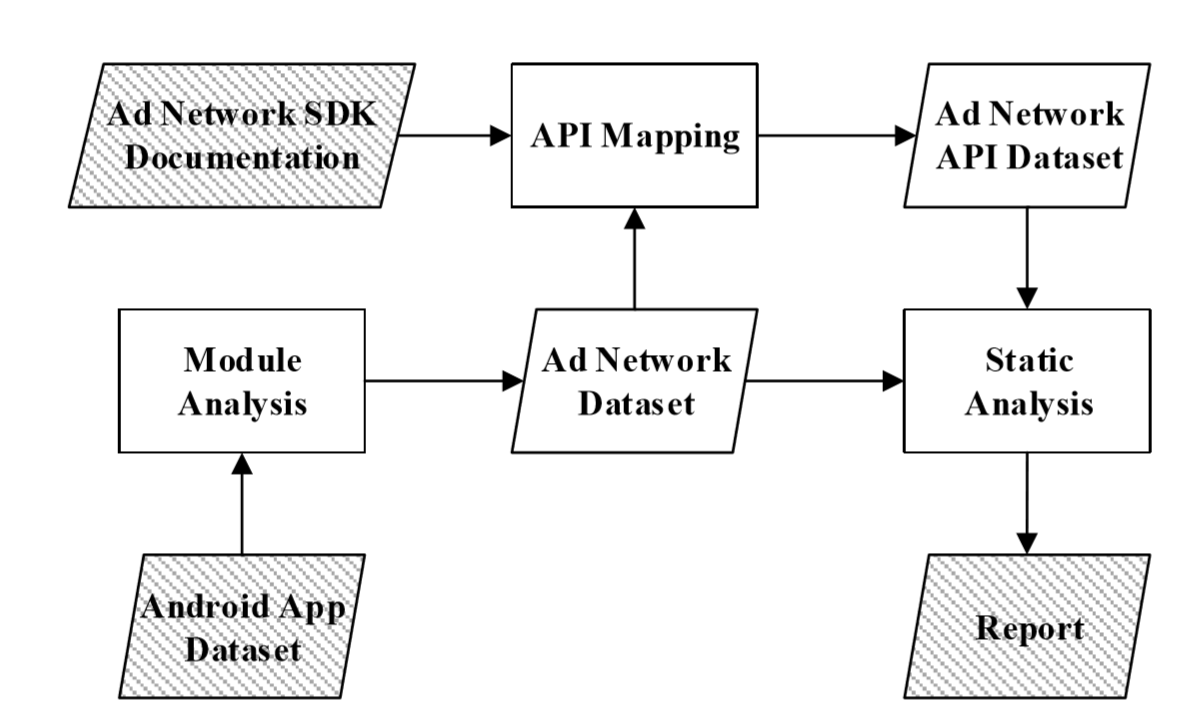
\includegraphics[width=0.5\textwidth,height=0.5\textheight,keepaspectratio]{system.png}
	\caption{Overview of MAdLens}
	\label{fig:system}
\end{figure}
The authors created MAdLens system (Fig. \ref{fig:system} ) which can identify internal third-party ad network modules from an Android app, map APIs of ad networks to specific ad types, and generate a detailed report of all the ad information for each app using static analysis techniques. Part of this system is a crawler that randomly picks applications from Google Play to create the Android App Dataset. For each application in the dataset, MAdLens automatically distinguishes all existing ad networks and then, using the API Mapping created based on Ad network SDK Documentation, classifies the present APIs in one of the five categories defined by the authors and generates an appropriate summary. To extract the relevant information from the applications, the system considers the fact that ads can be implemented either in the resource file (XML) or in Java code. For resources files, they decompile the apk file with Androidguard to get all the Android layout files, then parse all the XML to find the ads. Similarly, for Java code, the smali code is generated by Androguard after decompiling the apk file and ads are recognized in the smali text.

\section{Data Analysis and Results}
Steph

\section{Limitations and Future Work}
MAdLens takes the static approach of analyzing and extracting the APIs from Android applications. Therefore, it has the inherited limitation of static analysis. The system counts the number of occurrences of various APIs at a specific time and because of code control flow, some portions of the code are not necessarily executed. Thus, investigated apps could have had some other ads which were not captured because of this reason. There are dynamic approaches which can capture an app’s run-time behavior, but these are still very challenging to implement at a large scale. A viable alternative proposed in the paper was a dynamic solution to apply image recognition techniques to identify ad activities on the user interface. However, this option was left by the authors for future work as it requires significant additional research.

\section{Conclusion}
Steph




\bibliography{ref}
\bibliographystyle{IEEEtran}



\end{document}
